% --------------------------------------------------------------
% This is all preamble stuff that you don't have to worry about.
% Head down to where it says "Start here"
% --------------------------------------------------------------
 
\documentclass[12pt]{article}
 
\usepackage[margin=1in]{geometry} 
\usepackage{amsmath,amsthm,amssymb}
\usepackage{mathtools}
\usepackage{multicol}
\usepackage{textcomp}
\usepackage{float}
\usepackage{longtable}
\usepackage{hyperref}
 
\newcommand{\N}{\mathbb{N}}
\newcommand{\Z}{\mathbb{Z}}
\newcommand\aug{\fboxsep=-\fboxrule\!\!\!\fbox{\strut}\!\!\!}
 
\newenvironment{theorem}[2][Theorem]{\begin{trivlist}
\item[\hskip \labelsep {\bfseries #1}\hskip \labelsep {\bfseries #2.}]}{\end{trivlist}}
\newenvironment{lemma}[2][Lemma]{\begin{trivlist}
\item[\hskip \labelsep {\bfseries #1}\hskip \labelsep {\bfseries #2.}]}{\end{trivlist}}
\newenvironment{exercise}[2][Exercise]{\begin{trivlist}
\item[\hskip \labelsep {\bfseries #1}\hskip \labelsep {\bfseries #2.}]}{\end{trivlist}}
\newenvironment{reflection}[2][Reflection]{\begin{trivlist}
\item[\hskip \labelsep {\bfseries #1}\hskip \labelsep {\bfseries #2.}]}{\end{trivlist}}
\newenvironment{proposition}[2][Proposition]{\begin{trivlist}
\item[\hskip \labelsep {\bfseries #1}\hskip \labelsep {\bfseries #2.}]}{\end{trivlist}}
\newenvironment{corollary}[2][Corollary]{\begin{trivlist}
\item[\hskip \labelsep {\bfseries #1}\hskip \labelsep {\bfseries #2.}]}{\end{trivlist}}
 
\begin{document}
 
% --------------------------------------------------------------
%                         Start here
% --------------------------------------------------------------
 
%\renewcommand{\qedsymbol}{\filledbox}
 

% --------------------------------------------------------------
%     You don't have to mess with anything below this line.
% --------------------------------------------------------------
% --------------------------------------------------------------
% This is all preamble stuff that you don't have to worry about.
% Head down to where it says "Start here"
% --------------------------------------------------------------
 

% --------------------------------------------------------------
%                         Start here
% --------------------------------------------------------------
 
%\renewcommand{\qedsymbol}{\filledbox}

\title{TUTORIAL 10 - More recaps}%replace X with the appropriate number
\author{TRISTAN GLATARD\\ %replace with your name
COMP 361 Numerial Methods} %if necessary, replace with your course title
\date{November 23, 2018} 
\maketitle

\begin{exercise}{1} %You can use theorem, proposition, exercise, or reflection here. 

\begin{figure}[h]
    \centering
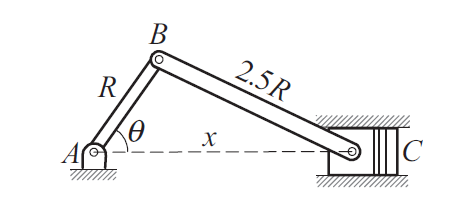
\includegraphics{5-1-12.png}
\end{figure}

The crank AB of length R = 90 mm is rotating at a constant angular speed of $d\theta/dt = 5 000$ rev/min. The position of the piston C can be shown to vary with
the angle $\theta$ as
$$x=R(cos\theta + \sqrt{2.5^2-sin^2\theta})$$
Use numerical differentiation to compute the acceleration at $\theta=0^0, 5^0, 10^0$

\textbf{Solution.} 
The acceleration is the second derivative of $x = f(\theta)= R(cos\theta + \sqrt{2.5^2-sin^2\theta})$. We will use central different approximation to calculate the acceleration at $\theta=0^0, 5^0, 10^0$ with $h=0.1$ (radian!) and $R = 0.09$ m. In this case, the approximation has the form:
$$f^{\prime\prime}(\theta) \approx \frac{f(\theta-h) -2f(\theta) + f(\theta+h)}{h^2}$$
Calculations are on the following table, note that we need to convert $\theta$ from degree to radian.

\begin{table}[h]
\centering
\begin{tabular}{|rrrrrr|}
\hline
\multicolumn{1}{|c}{\textbf{$\theta$(deg)}} & \multicolumn{1}{c}{\textbf{$\theta$(rad)}} & \multicolumn{1}{c}{\textbf{$f(\theta-h)$}} & \multicolumn{1}{c}{\textbf{$f(\theta)$}} & \multicolumn{1}{c}{\textbf{$f(\theta+h)$}} & \multicolumn{1}{c|}{\textbf{$f^{\prime\prime}(\theta)$}} \\ \hline
0 & 0.0000 & 0.3144 & 0.3150 & 0.3144 & -0.1258 \\
5 & 0.0873 & 0.3150 & 0.3145 & 0.3128 & -0.1250 \\
10 & 0.1745 & 0.3147 & 0.3131 & 0.3103 & -0.1225 \\ \hline
\end{tabular}
\end{table}

\end{exercise}

%EXERCISE 2-----------------------------------------------------
\begin{exercise}{2} %You can use theorem, proposition, exercise, or reflection here.  

The following table shows the power P supplied to the driving wheels of a car as a
function of the speed v. If the mass of the car is m = 2000 kg, determine the time
$\Delta t$ it takes for the car to accelerate from 1 m/s to 6 m/s. Use the trapezoidal rule
for integration. Hint: 	$\Delta t = m \int_{1s}^{6s}(v/P)dv$ , which can be derived from Newton’s
law $F = m(dv/dt)$ and the definition of power $P = Fv$.

\begin{table}[h]
\centering
\begin{tabular}{|c|c|c|c|c|c|c|c|c|c|c|c|}
\hline
v (m/s) & 0& 1.0& 1.8& 2.4& 3.5& 4.4& 5.1& 6.0\\ \hline
P (kW) &0 &4.7& 12.2 &19.0& 31.8& 40.1& 43.8 &43.2 \\ \hline
\end{tabular}
\end{table}

\textbf{Solution.}


Let f(v) = v/P, we transform the given table into 
\begin{table}[h]
\centering
\begin{tabular}{|c|c|c|c|c|c|c|c|c|c|c|c|}
\hline
v (m/s) & 0& 1.0& 1.8& 2.4& 3.5& 4.4& 5.1& 6.0\\ \hline
$f(v)*10^{-3}$ &0 &0.2128&	0.1475&	0.1263&	0.1101	&0.1097&0.1164	&0.1389
 \\ \hline
\end{tabular}
\end{table}

Apply trapezoidal rule on each panel,

\begin{table}[h]
\centering
\begin{tabular}{|rrrrrr|}
\hline
\multicolumn{1}{|c}{\textbf{a}} & \multicolumn{1}{c}{\textbf{b}} & \multicolumn{1}{c}{\textbf{h}} & \multicolumn{1}{c}{\textbf{$f(a)*10^{-3}$}} & \multicolumn{1}{c}{\textbf{$f(b)*10^{-3}$}} & \multicolumn{1}{c|}{\textbf{$I*10^{-3}$}} \\ \hline
1 & 1.8 & 0.8 & 0.2128 & 0.1475 & 0.14412 \\
1.8 & 2.4 & 0.6 & 0.1475 & 0.1263 & 0.08214 \\
2.4 & 3.5 & 1.1 & 0.1263 & 0.1101 & 0.13002 \\
3.5 & 4.4 & 0.9 & 0.1101 & 0.1097 & 0.09891 \\
4.4 & 5.1 & 0.7 & 0.1097 & 0.1164 & 0.079135 \\
5.1 & 6 & 0.9 & 0.1164 & 0.1389 & 0.114885 \\ \hline
\end{tabular}
\end{table}

Hence,
\begin{align}
\Delta t &= m \int_{1s}^{6s}(v/P)dv \notag \\
        &=m \int_{1s}^{6s}f(v)dv \notag \\
        &\approx \sum I \notag \\
        &=2000*0.6492*10^{-3} \notag \\
        &=1.2984 (s) \notag
\end{align}
\end{exercise}


%EXERCISE 3-----------------------------------------------------
\begin{exercise}{3} %You can use theorem, proposition, exercise, or reflection here.  

Determine $\int_1^{\infty} (1+x^4)^{-1}dx$ with the trapezoidal rule using five panels and compare
the result with the "exact" integral 0.24375. Hint: use the transformation $x^3 = 1/t$. 
\textbf{Solution.}

Let $x^3 = 1/t$, we have $dx=d(t^{-1/3})=-\frac{1}{3}t^{-4/3}dt$

The given integral becomes
\begin{align}
I&=\int_1^0 (1+t^{-4/3})^{-1}(-\frac{1}{3}t^{-4/3})dt \notag \\
&=\frac{1}{3}\int_0^1 (1+t^{4/3})^{-1}dt \notag 
\end{align}

Apply trapezoidal rule on five panels, with h = 0.2 and $f(t) = (1+t^{4/3})^{-1}$ on [0,1], we have the approximation

% Please add the following required packages to your document preamble:
% \usepackage{graphicx}
\begin{table}[h]
\centering
\begin{tabular}{|crrrrr|}
\hline
\textbf{Panel} & \multicolumn{1}{c}{$x_i$} & \multicolumn{1}{c}{$x_{i+1}$} & \multicolumn{1}{c}{$f(x_{i+1)}$} & \multicolumn{1}{c}{$f(x_{i+1})$} & \multicolumn{1}{c|}{$I_{i}$} \\ \hline
1 & 0 & 0.2 & 1.00000 & 0.89528 & 0.18953 \\
2 & 0.2 & 0.4 & 0.89528 & 0.77236 & 0.16676 \\
3 & 0.4 & 0.6 & 0.77236 & 0.66398 & 0.14363 \\
4 & 0.6 & 0.8 & 0.66398 & 0.57384 & 0.12378 \\
5 & 0.8 & 1 & 0.57384 & 0.50000 & 0.10738 \\ \hline
\end{tabular}

\end{table}

Then,
$$I = \frac{1}{3}\sum_{i=1}^{5} I_i = 0.24370$$

The result is very close to the "exact" value of 0.24375
\end{exercise}


%EXERCISE 4-----------------------------------------------------
\begin{exercise}{4} %You can use theorem, proposition, exercise, or reflection here.  
In the following sets of coupled differential equations t is the independent variable.
Convert these equations into first-order equations of the form $\dot y = F(t,y)$
\begin{enumerate}
    \item $\ddot y=x-2y$ \qquad \qquad \qquad \qquad $\ddot x = y-x$  
    \item $\ddot y=-y(\dot y^2+\dot x^2)^{1/4}$ \qquad \qquad   $\ddot x = -x(\dot y^2+\dot x^2)^{1/4}-32$  
    \item $\ddot y^2+tsiny=4\dot x$ \qquad \qquad\qquad $x\ddot x + tcosy= 4\dot y$  
\end{enumerate}

\textbf{Solution.}
Let
        $$
        y=
        \begin{bmatrix}
        y_0\\ y_1\\ y_2 \\ y_3 
        \end{bmatrix}
        =
        \begin{bmatrix}
        x\\ \dot x \\  y \\ \dot y 
        \end{bmatrix}
        $$
        
\begin{enumerate}
    \item $$
        F_1(t,y)=
        \begin{bmatrix}
        \dot y_0\\ \dot y_1\\ \dot y_2 \\ \dot y_3
        \end{bmatrix}
        =
        \begin{bmatrix}
        y_1\\ y_2-y_0 \\ y_3  \\ y_0-2y_2 
        \end{bmatrix}
        $$
    \item $$
        F_2(t,y)=
        \begin{bmatrix}
        \dot y_0\\ \dot y_1\\ \dot y_2 \\ \dot y_3
        \end{bmatrix}
        =
        \begin{bmatrix}
        y_1\\ -y_0(y_3^2+y_1^2)^{1/4}-32 \\ y_3  \\ -y_2(y_3^2+y_1^2)^{1/4}
        \end{bmatrix}
        $$
    \item $$
        F_3(t,y)=
        \begin{bmatrix}
        \dot y_0\\ \dot y_1\\ \dot y_2 \\ \dot y_3
        \end{bmatrix}
        =
        \begin{bmatrix}
        y_1\\ \frac{4y_3-tcosy_2}{y_0} \\ y_3  \\  \sqrt{4y_1-tsiny_2}
        \end{bmatrix}
        $$
\end{enumerate}

\end{exercise}

%EXERCISE 5-----------------------------------------------------
\begin{exercise}{5} %You can use theorem, proposition, exercise, or reflection here.  
Use first central difference approximations to transform the boundary value problem into simultaneous equations $Ay = b$
$$y^{\prime\prime}=y+x^2, \quad y(0)=0, \quad y(1)=1$$
\textbf{Solution.}

First central difference approximations is given as
\begin{align}
y^\prime_i &= \frac{y_{i+1}-y_{i-1}}{2h} \notag \\
y^{\prime\prime}_i &= \frac{y_{i-1}-2y_i+y_{i+1}}{h^2} \notag
\end{align}

where $h=\frac{1}{m}$ (m is to be chosen) is step size

The problem becomes
\begin{align}
\frac{y_{i-1}-2y_i+y_{i+1}}{h^2} = y_i+x_i^2,\quad i=1,2,...m-1\notag \\
y_{i-1}-2y_i+y_{i+1} - {h^2}(y_i+x_i^2) = 0, \quad i=1,2,...m-1\notag \\
y_{i-1} - (2+h^2)y_i+y_{i+1} = h^2x_i^2 , \quad i=1,2,...m-1 \label{eq1}  \notag \\
y_{i-1} - (2+\frac{1}{m^4})y_i+y_{i+1} = \frac{i^2}{m^4} , \quad i=1,2,...m-1 \end{align}

where $x_i = i*h$

The boundary conditions become
\begin{align}
y_0 &= y(x_0)= y(0) = 0 \label{eq2} \\ 
y_m &= y(x_m)= y(1) = 1 \label{eq3} 
\end{align}

Finally, we have a system of \textit{m+1} of \textit{m+1} unknowns $y_i, i=0,1,..m$ equations given by (\ref{eq1}), (\ref{eq2}) and (\ref{eq3}).

\end{exercise}


 
% \documentclass[12pt]{article}

\usepackage[margin=1in]{geometry}
\usepackage{amsmath,amsthm,amssymb}
\usepackage{mathtools}
\usepackage{multicol}
\usepackage{textcomp}
\usepackage{float}
\usepackage{longtable}

\newcommand{\N}{\mathbb{N}}
\newcommand{\Z}{\mathbb{Z}}
\newcommand\aug{\fboxsep=-\fboxrule\!\!\!\fbox{\strut}\!\!\!}

\newenvironment{theorem}[2][Theorem]{\begin{trivlist}
\item[\hskip \labelsep {\bfseries #1}\hskip \labelsep {\bfseries #2.}]}{\end{trivlist}}
\newenvironment{lemma}[2][Lemma]{\begin{trivlist}
\item[\hskip \labelsep {\bfseries #1}\hskip \labelsep {\bfseries #2.}]}{\end{trivlist}}
\newenvironment{exercise}[2][Exercise]{\begin{trivlist}
\item[\hskip \labelsep {\bfseries #1}\hskip \labelsep {\bfseries #2.}]}{\end{trivlist}}
\newenvironment{reflection}[2][Reflection]{\begin{trivlist}
\item[\hskip \labelsep {\bfseries #1}\hskip \labelsep {\bfseries #2.}]}{\end{trivlist}}
\newenvironment{proposition}[2][Proposition]{\begin{trivlist}
\item[\hskip \labelsep {\bfseries #1}\hskip \labelsep {\bfseries #2.}]}{\end{trivlist}}
\newenvironment{corollary}[2][Corollary]{\begin{trivlist}
\item[\hskip \labelsep {\bfseries #1}\hskip \labelsep {\bfseries #2.}]}{\end{trivlist}}

\begin{document}

\title{TUTORIAL 2}
\author{Timothée Guédon \& Tristan Glatard\\
COMP 361 Numerical Methods}
\date{September 20, 2019}
\maketitle

\section{Exercises for today}

\begin{exercise}{1}
Invert the following matrix using Gauss elimination or Gauss-Jordan elimination:
\begin{center}
\textbf{B}=
$
\begin{bmatrix}
2 & -2 & 1 \\
1 & 0 & -1 \\
4 & 1 & 1
\end{bmatrix}
$
\end{center}
\end{exercise}

\begin{exercise}{2}
Find Doolittle's LU decomposition of \textbf{B}:\\
\begin{center}
\textbf{B}=
$
\begin{bmatrix}
2 & -2 & 1 \\
1 & 0 & -1 \\
4 & 1 & 1
\end{bmatrix}$
\end{center}
Then solve $Bx=b$ for $b = \begin{bmatrix}
  1 \\ 2 \\ 0
\end{bmatrix}$
\end{exercise}

\begin{exercise}{3}
Find the Cholesky decomposition of \textbf{A}: \\
\begin{center}
\textbf{A}=
$
\begin{bmatrix}
1 & 1 & 1 \\
1 & 2 & 2 \\
1 & 2 & 3
\end{bmatrix}
$
\end{center}
\end{exercise}

\begin{exercise}{4} (As a training)
Invert the following matrix:
\begin{center}
\textbf{D}=
$
\begin{bmatrix}
3 & 1 & 2 \\
1 & 1 & 0 \\
5 & 8 & 9
\end{bmatrix}
$
\end{center}
\end{exercise}

\break

\section{Solutions}

%-------------------------------------------------------------------------------------------------------
\subsection{Exercise 1}
%-------------------------------------------------------------------------------------------------------

\textbf{Gauss elimination} \\

\begin{center}
\textbf{[$B \vert I$]}=
$\begin{bmatrix}
2 & -2 & 1 & \aug & 1 & 0 & 0 \\
1 & 0 & -1 & \aug & 0 & 1 & 0 \\
4 & 1 & 1 & \aug & 0 & 0 & 1 \\
\end{bmatrix}
$
\end{center}

\noindent $L_1 \gets L_3$ \\
$L_3 \gets L_1$ \\
\begin{center}
$\begin{bmatrix}
4 & 1 & 1 & \aug & 0 & 0 & 1 \\
1 & 0 & -1 & \aug & 0 & 1 & 0 \\
2 & -2 & 1 & \aug & 1 & 0 & 0 \\
\end{bmatrix}$
\end{center}

\noindent $L_1 \gets L_1/4$ \\
\begin{center}
$\begin{bmatrix}
1 & \frac{1}{4} & \frac{1}{4} & \aug & 0 & 0 & \frac{1}{4} \\
1 & 0 & -1 & \aug & 0 & 1 & 0 \\
2 & -2 & 1 & \aug & 1 & 0 & 0 \\
\end{bmatrix}$
\end{center}

\noindent $L_2 \gets L_2 - L_1$ \\
$L_3 \gets L_3 - 2 * L_1$ \\
\begin{center}
$\begin{bmatrix}
1 & \frac{1}{4} & \frac{1}{4} & \aug & 0 & 0 & \frac{1}{4} \\
0 & \frac{-1}{4} & \frac{-5}{4} & \aug & 0 & 1 & \frac{-1}{4} \\
0 & \frac{-10}{4} & \frac{2}{4} & \aug & 1 & 0 & \frac{-2}{4} \\
\end{bmatrix}$
\end{center}

\noindent $L_3 \gets L_3 - 10 * L_2$ \\
\begin{center}
$\begin{bmatrix}
1 & \frac{1}{4} & \frac{1}{4} & \aug & 0 & 0 & \frac{1}{4} \\
0 & \frac{-1}{4} & \frac{-5}{4} & \aug & 0 & 1 & \frac{-1}{4} \\
0 & 0 & 13 & \aug & 1 & -10 & \frac{8}{4} \\
\end{bmatrix}$
\end{center}


\noindent $L_3 \gets L_3/13$ \\
\begin{center}
$\begin{bmatrix}
1 & \frac{1}{4} & \frac{1}{4} & \aug & 0 & 0 & \frac{1}{4} \\
0 & \frac{-1}{4} & \frac{-5}{4} & \aug & 0 & 1 & \frac{-1}{4} \\
0 & 0 & 1 & \aug & \frac{1}{13} & \frac{-10}{13} & \frac{2}{13} \\
\end{bmatrix}$
\end{center}

\noindent For the Gauss elimination method, we stop here and we solve the following system of equations by backward substitution for each vector $b$ in the augmented matrix: \\
$$\begin{cases}
  a + \frac{1}{4}b + \frac{1}{4}c = b_1 \\
  \frac{-1}{4}b + \frac{-5}{4}c = b_2 \\
  c = b_3
\end{cases}$$ \\

with $$ b = \begin{bmatrix}
  0 \\
  0 \\
  \frac{1}{13}
\end{bmatrix} b = \begin{bmatrix}
  0 \\
  1 \\
  \frac{-10}{13}
\end{bmatrix} b = \begin{bmatrix}
  \frac{1}{4} \\
  \frac{-1}{4} \\
  \frac{2}{13}
\end{bmatrix} $$ \\

You should then find: \\

$$B^{-1} = \frac{1}{52}
\begin{bmatrix}
4 & 12 & 8 & \\
-20 & -8 & 12 \\
4 & -40 & 8
\end{bmatrix}$$ \\

\noindent \textbf{Gauss-Jordan elimination} \\
Gauss-Jordan elimination is just the Gauss elimination taken to its limit: When $U$ is found, you can continue the elimination on $U$ with pivots from $U_{N, N}$ to $U_{N-1, N-1}$.\\

\noindent $L_2 \gets L_2 + \frac{5}{4}L_3$ \\
$L_1 \gets L_1 - \frac{1}{4}L_3$ \\
\begin{center}
$\begin{bmatrix}
1 & \frac{1}{4} & 0 & \aug & \frac{-1}{52} & \frac{10}{52} & \frac{11}{52} \\
0 & \frac{-1}{4} & 0 & \aug & \frac{5}{52} & \frac{2}{52} & \frac{-3}{52} \\
0 & 0 & 1 & \aug & \frac{1}{13} & \frac{-10}{13} & \frac{2}{13} \\
\end{bmatrix}$
\end{center}

\noindent $L_1 \gets L_1 + L_2$ \\
\begin{center}
$\begin{bmatrix}
1 & 0 & 0 & \aug & \frac{4}{52} & \frac{12}{52} & \frac{8}{52} \\
0 & \frac{-1}{4} & 0 & \aug & \frac{5}{52} & \frac{2}{52} & \frac{-3}{52} \\
0 & 0 & 1 & \aug & \frac{1}{13} & \frac{-10}{13} & \frac{2}{13} \\
\end{bmatrix}$
\end{center}

\noindent $L_2 \gets (-4)*L_2$ \\
\begin{center}
\textbf{[$I \vert B^{-1}$]}=$\begin{bmatrix}
1 & 0 & 0 & \aug & \frac{4}{52} & \frac{12}{52} & \frac{8}{52} \\
0 & 1 & 0 & \aug & \frac{-20}{52} & \frac{-8}{52} & \frac{12}{52} \\
0 & 0 & 1 & \aug & \frac{4}{52} & \frac{-40}{52} & \frac{8}{52} \\
\end{bmatrix}$
\end{center}

We have found the same $B^{-1}$ as with the Gauss elimination. Let's test if our solution is right: \\

\begin{center}
$BB^{-1}=\begin{bmatrix}
2 & -2 & 1 \\
1 & 0 & -1 \\
4 & 1 & 1
\end{bmatrix}\frac{1}{52}
\begin{bmatrix}
4 & 12 & 8 & \\
-20 & -8 & 12 \\
4 & -40 & 8
\end{bmatrix} = \frac{1}{52}
\begin{bmatrix}
52 & 0 & 0 \\
0 & 52 & 0 \\
0 & 0 & 52
\end{bmatrix} = I
$
\end{center}

%-------------------------------------------------------------------------------------------------------
\subsection{Exercise 2}
%-------------------------------------------------------------------------------------------------------

\begin{center}
\textbf{B}=$\begin{bmatrix}
2 & -2 & 1 \\
1 & 0 & -1 \\
4 & 1 & 1
\end{bmatrix}$
\end{center}\\

Doolittle's decomposition is obtained through Gauss elimination by storing multipliers in the lower part of B. \\
$L_2 \gets L_2 - \frac{1}{2} L_1 \\
L_3 \gets L_3 - 2L_1 $ \\
\begin{center}
\textbf{B}=
$\begin{bmatrix}
2&-2&1\\
\boxed{\frac{1}{2}}&1&-\frac{3}{2}\\
\boxed{2}&5&-1
\end{bmatrix}
$
\end{center}
$L_3 \gets L_3 - 5L_2 \\$
\begin{center}
\textbf{[L\textbackslash U]}=
$\begin{bmatrix}
2&-2&1\\
\boxed{\frac{1}{2}}&1&-\frac{3}{2}\\
\boxed{2}&\boxed{5}&\frac{13}{2}
\end{bmatrix}
$
\end{center}
Thus,
\begin{center}
\textbf{L}=
$\begin{bmatrix}
1&0&0\\
\frac{1}{2}&1&0\\
2&5&1
\end{bmatrix}
$
\textbf{U}=
$\begin{bmatrix}
2&-2&1\\
0&1&-\frac{3}{2}\\
0&0&\frac{13}{2}
\end{bmatrix}
$
\end{center}

\noindent Now we can solve for $b$: \\
1. Solve $Ly = b$ by forward substitution
\begin{itemize}
\item $y_1 = 1$
\item $\frac{1}{2}y_1 + y_2=2 \Rightarrow y_2=\frac{3}{2}$
\item $2y_1+5y_2+y_3=0 \Rightarrow y_3=-\frac{19}{2}$
\end{itemize}
2. Solve $Ux = y$ by backward substitution
\begin{itemize}
\item $\frac{13}{2}x_3=-\frac{19}{2} \Rightarrow x_3=-\frac{19}{13}$
\item $x_2-\frac{3}{2}x_3=\frac{3}{2} \Rightarrow x_2=-\frac{9}{13}$
\item $2x_1-2x_2+x_3=1 \Rightarrow x_1=\frac{1}{2}(1-\frac{18}{13}+\frac{19}{13})=\frac{7}{13}$
\end{itemize}


%-------------------------------------------------------------------------------------------------------
\subsection{Exercise 3}
%-------------------------------------------------------------------------------------------------------

\begin{center}
\textbf{A}=
$\begin{bmatrix}
1&1&1\\
1&2&2\\
1&2&3
\end{bmatrix}
$
\end{center}

\begin{center}
$\textbf{A}= LL^T =
\begin{bmatrix}
L_{11}&0&0\\
L_{21}&L_{22}&0\\
L_{31}&L_{32}&L_{33}\\
\end{bmatrix}
\begin{bmatrix}
L_{11}&L_{21}&L_{31}\\
0&L_{22}&L_{32}\\
0&0&L_{33}\\
\end{bmatrix}
$
\end{center}

Identification of column 1:
\begin{itemize}
\item $L_{11} = 1$
\item $L_{11}L_{21} = 1 \Rightarrow L_{21} = 1$
\item $L_{11}L_{31} = 1 \Rightarrow L_{31} = 1$
\end{itemize}

Identification of column 2:
\begin{itemize}
\item $L_{21}^2 + L_{22}^2 = 2 \Rightarrow L_{22} = 1$
\item $1+L_{22}L_{32} = 2 \Rightarrow L_{32} = 1$
\end{itemize}

Identification of column 3:
\begin{itemize}
\item $L_{31}^2 + L_{32}^2  + L_{33}^2 = 3 \Rightarrow L_{33} = 1$
\end{itemize}

Therefore,
\begin{center}
\textbf{L}=
$\begin{bmatrix}
1&0&0\\
1&1&0\\
1&1&1
\end{bmatrix}
$
\end{center}

\subsection{Exercise 4}
\textbf{Using Gauss elimination}

\noindent We will solve $DX=I$ by Gauss elimination \\

\begin{center}
\textbf{[$D \vert I$]}=
$\begin{bmatrix}
3&1&2 &\aug&1&0&0\\
1&1&0 &\aug& 0&1&0\\
5&8&9 &\aug& 0&0&1
\end{bmatrix}
$ \\
\end{center}

\noindent $L_2 \leftarrow L_2 - \frac{1}{3}L_1$\\
$L_3 \leftarrow L_3 - \frac{5}{3}L_1$\\

\begin{center}
$\begin{bmatrix}
3&1&2 &\aug&1&0&0\\
0&\frac{2}{3}&-\frac{2}{3} &\aug&-\frac{1}{3}&1&0\\
0&\frac{19}{3}&\frac{17}{3} &\aug& -\frac{5}{3}&0&1
\end{bmatrix}
$ \\
\end{center}

$L_3 \leftarrow L_3 - \frac{19}{2}L_2$\\

\begin{center}
$\begin{bmatrix}
3&1&2 &\aug&1&0&0\\
0&\frac{2}{3}&-\frac{2}{3} &\aug&-\frac{1}{3}&1&0\\
0&0&12 &\aug& \frac{3}{2}&-\frac{19}{2}&1
\end{bmatrix}
$ \\
\end{center}

Back substitution
\begin{itemize}
\item $12x_{31} = \frac{3}{2} \Rightarrow x_{31} = -\frac{1}{8}$
\item $\frac{2}{3}x_{21} = -\frac{1}{3} + \frac{2.1}{3.8} \Rightarrow x_{21} = -\frac{3}{8}$
\item $x_{11} = \frac{1}{3}(1+\frac{3}{8}-\frac{2}{8}) = \frac{3}{8}$
\end{itemize}

\begin{itemize}
\item $12x_{32} = -\frac{19}{2} \Rightarrow x_{32} = -\frac{19}{24}$
\item $x_{22} = -\frac{3}{2}(1-\frac{2}{3}.\frac{19}{24}) = -\frac{17}{24}$
\item $x_{12} = \frac{1}{3}(0-\frac{17}{24}+2\frac{19}{24}) = \frac{7}{24}$
\end{itemize}

\begin{itemize}
\item $12x_{33} = 1 \Rightarrow x_{33} = \frac{1}{12}$
\item $x_{23} = -\frac{3}{2}(0+\frac{2}{3}.\frac{1}{12}) = \frac{1}{12}$
\item $x_{13} = \frac{1}{3}(0-\frac{1}{12}-\frac{2}{12}) = -\frac{1}{12}$
\end{itemize}

Finally,
\begin{center}
$C^{-1} = \begin{bmatrix}
\frac{3}{8} & \frac{7}{24} & \frac{-1}{12} \\
\frac{-3}{8} & \frac{17}{24} & \frac{1}{12} \\
\frac{1}{8} & \frac{-19}{24} & \frac{1}{12} \\
\end{bmatrix}
$
\end{center}

\end{document}
 
% % --------------------------------------------------------------
% This is all preamble stuff that you don't have to worry about.
% Head down to where it says "Start here"
% --------------------------------------------------------------
 

% --------------------------------------------------------------
%                         Start here
% --------------------------------------------------------------
 
%\renewcommand{\qedsymbol}{\filledbox}

\title{TUTORIAL 9 - Recap}%replace X with the appropriate number
\author{TRISTAN GLATARD\\ %replace with your name
COMP 361 Numerial Methods} %if necessary, replace with your course title
\date{November 16, 2018} 
\maketitle

\begin{exercise}{1} %You can use theorem, proposition, exercise, or reflection here. 
Use Gauss elimination to solve $\textbf{AX}=\textbf{B}$, where:
\begin{center}
\textbf{A}= 
$\begin{bmatrix}
2&0&-1&0\\ 
0&1&2&0\\
-1&2&0&1\\
0&0&1&-2
\end{bmatrix}
$ 
\textbf{B}= 
$\begin{bmatrix}
1&0\\ 0&0\\ 0&1 \\ 0&0
\end{bmatrix}
$ 
\end{center}

\textbf{Solution.} 

$(3) \longleftarrow (1) + 2*(3)$

\begin{center}
\textbf{[$A \vert B$]}= 
$\begin{bmatrix}
2&0&-1&0 &\aug & 1 & 0\\ 
0&1&2&0 &\aug & 0 & 0\\
0&4&-1&2&\aug & 1 & 2\\
0&0&1&-2&\aug & 0 & 0
\end{bmatrix}
$ 
\end{center}

$(3) \longleftarrow 4*(2) - (3)$
\begin{center}
\textbf{[$A \vert B$]}= 
$\begin{bmatrix}
2&0&-1&0 &\aug & 1 & 0\\ 
0&1&2&0 &\aug & 0 & 0\\
0&0&9&-2&\aug & -1 & -2\\
0&0&1&-2&\aug & 0 & 0
\end{bmatrix}
$ 
\end{center}

$(4) \longleftarrow (3) - 9*(4)$
\begin{center}
\textbf{[$A \vert B$]}= 
$\begin{bmatrix}
2&0&-1&0 &\aug & 1 & 0\\ 
0&1&2&0 &\aug & 0 & 0\\
0&0&9&-2&\aug & -1 & -2\\
0&0&0&16&\aug & -1 & -2
\end{bmatrix}
$ 
\end{center}

First solve $Ax_1=B_1$, where 

$$B_1= 
\begin{bmatrix}
1\\ 0\\ -1 \\ -1
\end{bmatrix}
$$ 

\begin{itemize}
    \item $16x_{41} = -1 \Longrightarrow x_{41} = -\frac{1}{16}$ 
    \item $9x_{31} - 2x_{41} = -1 \Longrightarrow x_{31} = -\frac{1}{8}$ 
    \item $x_{21} + 2x_{31} = 0 \Longrightarrow x_{21} = \frac{1}{4}$ 
    \item $2x_{11} - x_{31} = 1 \Longrightarrow x_{11} = \frac{7}{16}$ 
\end{itemize}

Then solve $Ax_1=B_2$, where 

$$B_2= 
\begin{bmatrix}
0\\ 0\\ -2 \\ -2
\end{bmatrix}
$$ 

\begin{itemize}
    \item $16x_{42} = -2 \Longrightarrow x_{41} = -\frac{1}{8}$ 
    \item $9x_{32} - 2x_{42} = -2 \Longrightarrow x_{32} = -\frac{1}{4}$ 
    \item $x_{22} + 2x_{32} = 0 \Longrightarrow x_{22} = \frac{1}{2}$ 
    \item $2x_{12} - x_{32} = 1 \Longrightarrow x_{11} = \frac{3}{8}$ 
\end{itemize}

Finally the solution is
$$x= 
\begin{bmatrix}
\frac{7}{16} & \frac{3}{8}\\ 
\frac{1}{4} & \frac{1}{2}\\ 
-\frac{1}{8} & -\frac{1}{4}\\ 
-\frac{1}{16} & -\frac{1}{8}
\end{bmatrix}
$$ 

\end{exercise}

%EXERCISE 2-----------------------------------------------------
\begin{exercise}{2} %You can use theorem, proposition, exercise, or reflection here.  
Using Doolittle\textquotesingle s decomposition, find L and U so that
\begin{center}
\textbf{A = LU = }
$\begin{bmatrix}
4&-1&0\\ 
-1&4&-1\\
0&-1&4
\end{bmatrix}
$ 
\end{center}

\textbf{Solution.}
Doolittle\textquotesingle s decomposition is obtained through Gauss elimination by storing multipliers in the lower part of A \\
$
(2) \longleftarrow (2) + \frac{1}{4} *(1)\\
$
$$\textbf{A = LU = }
\begin{bmatrix}
4&-1&0\\ 
\boxed{-\frac{1}{4}}&\frac{15}{4}&-1\\
0&-1&4
\end{bmatrix}
$$ 

$
(3) \longleftarrow (3) + \frac{4}{15}*(2)\\
$
$$\textbf{A = LU = }
\begin{bmatrix}
4&-1&0\\ 
\boxed{-\frac{1}{4}}&\frac{15}{4}&-1\\
0&\boxed{-\frac{4}{15}} & \frac{56}{15}
\end{bmatrix}
$$ 
Then we have

$$\textbf{L =}
\begin{bmatrix}
1&0&0\\ 
-\frac{1}{4}&1&0\\
0&-\frac{4}{15} & 1
\end{bmatrix}
\textbf{U = }
\begin{bmatrix}
4&-1&0\\ 
0&\frac{15}{4}&-1\\
0&0 & \frac{56}{15}
\end{bmatrix}
$$ 

\end{exercise}


%EXERCISE 3-----------------------------------------------------
\begin{exercise}{3} %You can use theorem, proposition, exercise, or reflection here.  
Using Lagrange\textquotesingle s interpolation over three nearest-neighbor data points, find the zero of y(x) from the following data:
\begin{table}[h]
\centering
\begin{tabular}{|c|c|c|c|c|c|c|c|}
\hline
x & 0 & 0.5 & 1& 1.5& 2& 2.5& 3 \\ \hline
y & 1.8421& 2.4694 &2.4921& 1.9047& 0.8509 &-0.4112 &-1.5727 \\ \hline
\end{tabular}
\end{table}

\textbf{Solution.}
From the table, we have the root of y(x)=0 lies between [2,2.5].
Let\textquotesingle s try to use Lagrange\textquotesingle s to interpolate a polynomial that passes three nearest data points in the interval [1.5,2,2.5]

With 3 given data points, we can construct a degree-2 polynomial using the Lagrange formula:\\
$$P_{2}(x)=\sum_{i=0}^2 y_{i}\ell_{i}(x)$$
where
\begin{align}
\ell_{0}(x)&=\frac{(x-x_1)(x-x_2)}{(x_0-x_1)(x_0-x_2)}=\frac{(x-2)(x-2.5)}{(1.5-2)(1.5-2.5)} = 2x^2-9x+10 \notag\\
\ell_{1}(x)&=\frac{(x-x_0)(x-x_2)}{(x_1-x_0)(x_1-x_2)}=\frac{(x-1.5)(x-2.5)}{(2-1.5)(2-2.5)}= -4x^2 + 16x - 15 \notag\\
\notag 
\ell_{2}(x)&=\frac{(x-x_0)(x-x_1)}{(x_2-x_0)(x_2-x_1)}=\frac{(x-1.5)(x-2)}{(2.5-1.5)(2.5-2)} = 2x^2-7x + 7
\end{align}
Then
\begin{align}
P_{2}(x)&=\sum_{i=0}^2 y_{i}\ell_{i}(x) \notag \\
&= 1.9047(2x^2-9x+10) \notag \\
&+ 0.8509(-4x^2 + 16x - 15) \notag \\
&-0.4112(2x^2-7x + 7) \notag \\
&=-0.4166x^2-0.6495x+3.4051 \notag
\end{align}
The root of $P_2(x) = 0$ in the interval [2,2.5] is \textbf{2.1838}.

\end{exercise}


%EXERCISE 4-----------------------------------------------------
\begin{exercise}{4} %You can use theorem, proposition, exercise, or reflection here.  
Three tensile tests were carried out on an aluminum bar. In each test the strain was measured at the same values of stress. The results were given in the table where the units of strain are \textit{mm/m}. Use linear regression to estimate the modulus of elasticity of the bar (modulus of elasticity = stress/strain).

\begin{table}[h]
\centering
\begin{tabular}{|c|c|c|c|c|}
\hline
Stress (MPa) & 34.5& 69.0 &103.5 &138.0 \\ \hline
Strain (Test 1) &0.46& 0.95 &1.48& 1.93 \\ \hline
Strain (Test 2)& 0.34 &1.02 &1.51& 2.09 \\ \hline
Strain (Test 3) &0.73& 1.10& 1.62& 2.12 \\ \hline
\end{tabular}
\end{table}

\textbf{Solution.}
If we consider all tests have same weight, we have experiment data for stress and strain as in the Table \ref{tab:stress-strain}

\begin{table}[h]
\centering
\begin{tabular}{|c|c|c|c|c|c|c|c|c|c|c|c|c|}
\hline
Stress & 34.5& 69.0 &103.5 &138.0 & 34.5& 69.0 &103.5 &138.0 & 34.5& 69.0 &103.5 &138.0\\ \hline
Strain &0.46& 0.95 &1.48& 1.93 & 0.34 &1.02 &1.51& 2.09 &0.73& 1.10& 1.62& 2.12 \\ \hline
\end{tabular}
\caption{My caption}
\label{tab:stress-strain}
\end{table}
Apply linear regression on 12-points in Table \ref{linear-regression-calculation} with $\overline{x} = 86.25$.
We have $$b=\frac{\sum y_i(x_i-\overline{x})}{\sum x_i(x_i-\overline{x})} = \frac{265.13*10^{-3}}{17853.75} = 1.485*10^{-5}$$
Then, the modulus of elasticity is
$$E=\frac{1}{b}=\frac{1}{1.485*10^{-5}} \approx 67,339 (MPa)$$

\begin{table}[H]
\centering
\begin{tabular}{|rrrr|}
\hline
\multicolumn{1}{|c|}{\textbf{Stress ($x_i$)}} & \multicolumn{1}{c|}{\textbf{Strain($y_i*10^{-3}$)}} & \multicolumn{1}{c|}{\textbf{$y_i(x_i-\overline{x})*10^{-3}$}} & \multicolumn{1}{c|}{\textbf{$x_i(x_i-\overline{x})$}} \\ \hline
34.50 & 0.46 & -23.81 & -1785.38 \\
69.00 & 0.95 & -16.39 & -1190.25 \\
103.50 & 1.48 & 25.53 & 1785.38 \\
138.00 & 1.93 & 99.88 & 7141.50 \\
34.50 & 0.34 & -17.60 & -1785.38 \\
69.00 & 1.02 & -17.60 & -1190.25 \\
103.50 & 1.51 & 26.05 & 1785.38 \\
138.00 & 2.09 & 108.16 & 7141.50 \\
34.50 & 0.73 & -37.78 & -1785.38 \\
69.00 & 1.10 & -18.98 & -1190.25 \\
103.50 & 1.62 & 27.95 & 1785.38 \\
138.00 & 2.12 & 109.71 & 7141.50 \\ \hline
 &  & 265.13 & 17853.75 \\ \hline
\end{tabular}
\caption{Linear regression calculation}
\label{linear-regression-calculation}
\end{table}


\end{exercise}


%EXERCISE 5-----------------------------------------------------
\begin{exercise}{5} %You can use theorem, proposition, exercise, or reflection here.  
Using the Newton-Raphson method, determine the two roots of $$sinx + 3cosx-2 = 0$$ that lie in the interval (-2, 2).

\textbf{Solution.}

Here the Newton-Raphson formula is\\
\begin{align}
\notag
x \leftarrow x - \Delta x  
\end{align}

where
\begin{align}
\Delta x = \frac{f(x)}{f^\prime(x)} = \frac{sinx + 3cosx-2}{cosx-3sinx}
\end{align}

until $|\Delta| \leq \epsilon = 10e^{-4}$\\

Starting with x=-2, the calculations are shown on 
Table \ref{calculation1}

\begin{table}[h]
\centering
\begin{tabular}{|c|r|r|}
\hline
\textit{\textbf{Iteration}} & \multicolumn{1}{c|}{\textit{\textbf{x}}} & \multicolumn{1}{c|}{\textit{\textbf{$\Delta x$}}} \\ \hline
1 & -2.00000 & -1.79853 \\ \hline
2 & -0.20147 & 0.46782 \\ \hline
3 & -0.66929 & -0.10117 \\ \hline
4 & -0.56812 & -0.00379 \\ \hline
5 & -0.56433 & -0.00001 \\ \hline
\end{tabular}
\caption{Calculation starting with x=-2}
\label{calculation1}
\end{table}

and we have root $x_1 \approx -0.56433$

Starting with $x=2$, the calculations are shown on Table \ref{calculation2}

\begin{table}[h]
\centering
\begin{tabular}{|c|r|r|}
\hline
\textit{\textbf{Iteration}} & \multicolumn{1}{c|}{\textit{\textbf{x}}} & \multicolumn{1}{c|}{\textit{\textbf{$\Delta x$}}} \\ \hline
1 & 2.00000 & 0.74399 \\ \hline
2 & 1.25601 & 0.04730 \\ \hline
3 & 1.20870 & 0.00088 \\ \hline
4 & 1.20783 & 0.00000 \\ \hline
\end{tabular}
\caption{Calculation starting with x=2}
\label{calculation2}
\end{table}
and we have root $x_2 \approx 1.2078$

\end{exercise}


 
\end{document}